\section{Einführung in neoinstitutionalistische Finanzierungstheorie}

$\rightarrow$ Finanzierung unter asymmetrischer Information (kein vollkommener Kapitalmarkt)\\

\textbf{Grundgedanke der Neoklassik} (Gegenteil von Neoinstitution):
\begin{itemize}
	\item Reibungslos funktionierender Markt (vollständig und vollkommen)
	\item Preise für Zahlungsströme sind gegeben
	\item Symmetrische Informationsverteilung
\end{itemize}
$\rightarrow$ \textbf{First-Best-Lösung} ohne zusätzliche Transaktionskosten erreichbar

$\rightarrow$ Neoklassik kann nicht die Existenz bedeutender Institutionen erklären, wie z.B. Verträge, Gesetze, Rating-Agenturen, ...\\

\textbf{Moderne Finanzierungstheorie: Nutzenmaximierung}
\begin{itemize}
	\item Möglichst geringe Gegenleistung für Preis
	\item \textbf{Asymmetrische Informationsverteilung}: Vertragsparteien haben nicht die gleichen Informationen über die Konditionen des Tauschgeschäfts $\rightarrow$ Täuschung möglich
	\item Interessen der Vertragspartner können im Konflikt zueinander stehen
	\item Potentielles \textbf{opportunistisches Verhalten} $\rightarrow$ Bereitschaft bewusst falsche Angaben zu machen, Vereinbarungen zu missachten und gegen die Interessen des Vertragspartners zu verstoßen, solange es ihnen einen höheren Nutzen verspricht
\end{itemize}
$\rightarrow$ \textbf{Interessenkonflikt zwischen Vertragsparteien}:
\begin{itemize}
	\item Hidden characteristics (ASIV vor Vertragsabschluss)
	\item Hidden action (ASIV nach Vertragsabschluss)
	\item Nachverhandlungen
\end{itemize}
\bigskip
\textbf{Hidden Characteristics (Adverse Selection)}:
\begin{itemize}
	\item Vertragsparteien haben unterschiedliche Informationen über die Qualität bzw. Eigenschaften des Vertragsgegenstands, z.B. Gebrauchtwagenkauf
	\item Ohne institutionelle Regelungen kann sich Marktteilnehmer nur dadurch schützen, dass er sich vom Markt zurückzieht oder das Verhalten der anderen antizipiert 
	
	$\rightarrow$ Nur wenige Transaktionen findet statt $\rightarrow$ Unvollständiger Markt
\end{itemize}

\textbf{Hidden Action (Moral Hazard)}:
\begin{itemize}
	\item Informationsasymmetrie nach Vertragsabschluss $\rightarrow$ Verhalten einer Vertragspartei nach Vertragsabschluss ist unbeobachtbar (weicht vlt. vom vereinbarten Verhalten ab) und hat Auswirkungen auf Nutzen der anderen Partei
	\item \textbf{Beispiel}: Reduktion des Arbeitseinsatzes bei fixer Entlohnung von Managern
\end{itemize}

\textbf{Nachverhandlung}:
\begin{itemize}
	\item Vertragspartei tätigt nach Vertragsabschluss eine irreversible Investitionen $\rightarrow$ Andere Partei kann das ausnutzen, um die Vertragskonditionen nachträglich zu ihren Gunsten abzuändern
	\item \textbf{Beispiel}: Zulieferer baut ein Werk in unmittelbarer Nähe einer Autofabrik, um just-in-time	Produkte anzuliefern
\end{itemize}
\bigskip
\textbf{Wie kann man diesen Problemen entgegenwirken?}

\begin{itemize}
	\item \textbf{Screening}: Informationsbeschaffung vor Vertragsabschluss (z.B. Kfz-Mechaniker zum Autokauf mitnehmen)
	\item \textbf{Monitoring}: Kontrolle nach Vertragsabschluss (Bsp. Überwachung des Managements durch den Aufsichtsrat)
	\item Anreizkompatible Vertragsgestaltung, z.B. Garantiezusagen, Erfolgsabhängige Entlohnung, Optionsrechte (z.B. Mieter muss Wohnung bei Auszug sauber machen)
\end{itemize}

$\rightarrow$ Schutzmaßnahmen werden auch \textbf{Institutionen} genannt

$\rightarrow$ Verursachen \textbf{Transaktionskosten} (z.B. Kosten für Durchsetzen von Verträgen) $\rightarrow$ Keine First-Best-Lösung, sondern \textbf{Second-Best-Lösung}

\textbf{Agency-Kosten}: Differenz zwischen First-Best- und Second-Best-Lösung $\rightarrow$ Wohlfahrtsverlust, der aus den obigen Problemen resultiert\\

\textbf{Adverse Selection - Pecking Order Theorie}:
\begin{itemize}
	\item Anreiz, Aktien (EK) zu emittieren, wenn das Unternehmen überbewertet ist
	\item Kapitalmarktteilnehmer antizipieren den Anreiz des Managements und nehmen Kurskorrektur vor $\rightarrow$ \textbf{Negativer Ankündigungseffekt} (negative Aktienkursreaktion bei Bekanntgabe einer Kapitalerhöhung)
\end{itemize}

$\rightarrow$ Unterinvestition: Unternehmen, die am Kapitalmarkt richtig gepreist sind verzichten auf Investitionen, wenn die dafür notwendige EK-Erhöhung zu einem Wertverlust der Aktien führt, der den Ertrag übersteigt
\begin{itemize}
	\item FK ist von diesem Problem weniger stark betroffen, Innenfinanzierung gar nicht $\rightarrow$ Rangfolge (\textbf{Pecking Order}) von Finanzierungsformen
\end{itemize}
\bigskip
\textbf{Adverse Selection: Kreditvergabe \& Kreditsicherheiten}:
\begin{itemize}
	\item Bank will Betrag von 1000 in Projekt investieren und möchte erwarteten Gewinn über den risikolosen Zins von 0
	\item Risikoloser Zins ist 10\%
	\item Seien nun zwei Projekte gegeben:
	\begin{center}
		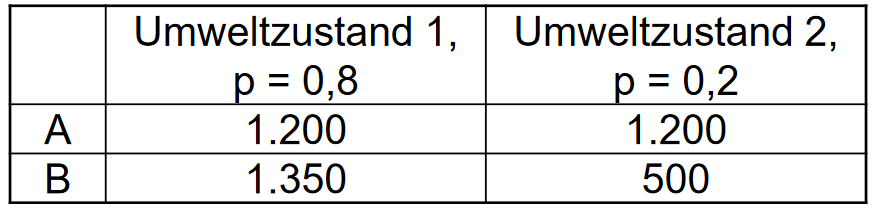
\includegraphics[width=0.4\textwidth]{images/as-1.png}
	\end{center} 
\end{itemize}
Zinssätze bei \underline{symmetrischer} Information:
\begin{itemize}
	\item Projekt A ist risikolos: 10\%
	\item Projekt B: $0,8\cdot 1000\cdot (1+i)+0,2\cdot 500=1100 \Rightarrow i=0,25$, d.h. Bank verlangt Zins in Höhe von 25\%, um im Mittel min. den risikolosen Zins zu erhalten
\end{itemize}
Bei Unbeobachtbarkeit des Projekttyps (\underline{ASIV}) für die Bank:
\begin{itemize}
	\item Sei $q$ der Anteil von Kunden mit risikolosem Projekt
	\item Maximale Zahlungsbereitschaft der Kreditnehmer beträgt:
	\begin{itemize}
		\item A: $1200-1000(1+i)\geq 0 \Rightarrow i\leq 0,2$
		\item B: $0,8(1350-1000(1+i))+0,2\cdot0\geq 0 \Rightarrow i\leq 0,35$
	\end{itemize}
	\item Damit Bank einen Gewinn von 0 erwirtschaftet, muss für die Zinssätze gelten:
	\begin{itemize}
		\item A: $1000(1+i)=1100\Leftrightarrow 1000i-100=0$
		\item B: $0,8\cdot 1000\cdot (1+i)+0,2\cdot 500=1100\Leftrightarrow 800i-200=0$
	\end{itemize}
	\item Damit folgt: $q(1000i-100)+(1-q)(800i-200)=0\Rightarrow i=\frac{2-q}{8+2q}$
	\item Bank muss beachten, dass ab einem Zinssatz von 20\% die risikolosen Unternehmer keinen Kredit mehr nachfragen. Kritischer Wert für $q$:
	$\frac{2-q}{8+2q}=0,2\Rightarrow q^*=0,286$
	\item Ist $q$ geringer, werden keine risikolosen Projekte mehr finanziert und der Zins steigt sofort auf 25\%
\end{itemize}
$\rightarrow$ \textbf{Problem}: Verdrängung der guten (risikolosen) Kreditnehmer vom Markt (\textbf{adverse Selektion})
\begin{center}
	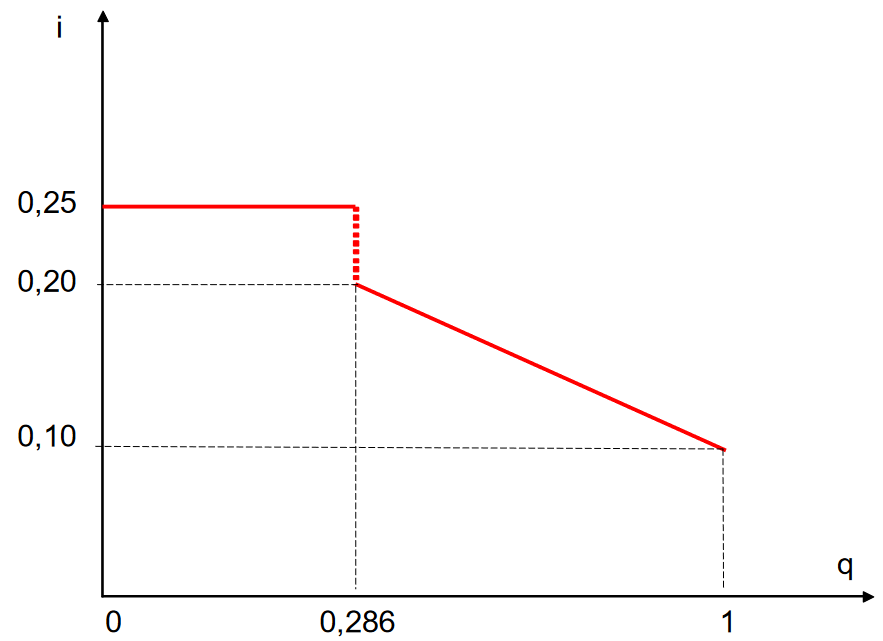
\includegraphics[width=0.4\textwidth]{images/as-2.png}
\end{center} 

Lösungsmöglichkeit: \textbf{Kreditsicherheiten}
\begin{itemize}
	\item Unternehmer können Kreditsicherheiten im subjektiven Wert von 700 anbieten
	\item Bei Verwertung der Sicherheit (wenn Kredit nicht zurückgezahlt werden kann) werden nur 600 von der Bank erlöst
	\item Bank könnte zwei Verträge anbieten:
	\begin{itemize}
		\item Kreditsicherheiten und einen Zins von 10\%
		\item Keine Sicherheiten und einen Zins von 25\%
	\end{itemize}
	$\rightarrow$ Beide Projekte werden so für die Bank risikolos, da wenn B den ersten Vertrag wählt und der schlechte Fall eintritt gilt: $500+600=1100$
	\item A wird Vertrag 1 wählen, da A die Sicherheiten sicher zurückbekommt und so nur einen Zins von 10\% zahlen muss
	\item B wird Vertrag 2 wählen, denn:
	\begin{itemize}
		\item Gewinn bei Vertrag 1: $0,8(1350-1100)+0,2(-700)=60$
		\item Gewinn bei Vertrag 2: $0,8(1350-1250)+0,2\cdot 0=80$
	\end{itemize}
\end{itemize}

$\rightarrow$ Selbstselektion (Angebot der Bank so, dass Kreditnehmer seinen Typ offenbart) aufgrund eines trennenden Gleichgewichts (\textbf{separating equilibrium})\\

\textbf{Moral Hazard: Asset Substitution}:
\begin{itemize}
	\item Moral-Hazard Problematik zwischen Eigentümern und Fremdkapitalgebern
	\item EK-Geber werden vom Cash-Flow (CF) erst bedient, wenn FK-Geber bedient wurden
	\item EK-Geber haben Interesse Risiko der Investition zum Nachteil der FK-Geber (höheres Insolvenzrisiko) tu erhöhen $\rightarrow$ \textbf{Asset-Substitution Problem}
	\begin{center}
		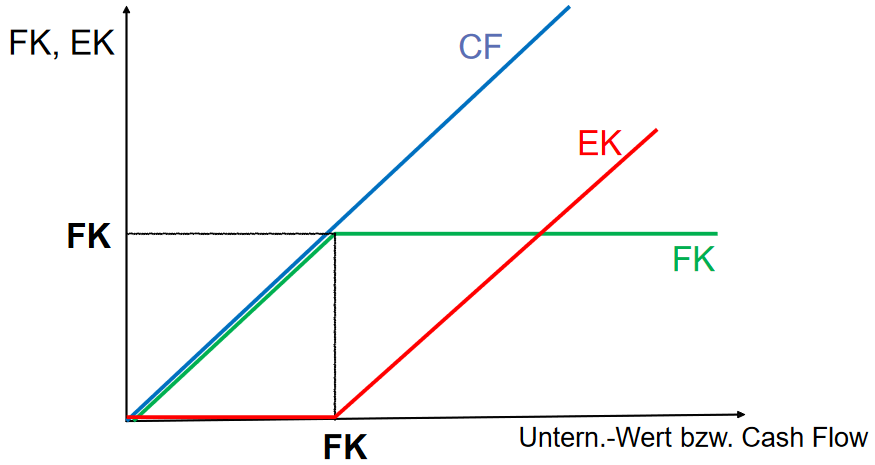
\includegraphics[width=0.4\textwidth]{images/mh.png}
	\end{center} 
	\item \textbf{Grund}: Wenn sicheres Investment zu einem Wert links von FK führt bekommen EK-Geber nix. Bei Risiko kann der Wert aber mit einer bestimmten W'keit rechts von FK sein und die EK-Geber erhalten etwas
\end{itemize}

\textbf{Beispiel}:
\begin{itemize}
	\item Bank leiht Unternehmen 1000, risikoloser Zins ist 10\%
	\item Unternehmen kann sich nun entscheiden, ob er Projekt A oder B ausführt
	\begin{center}
		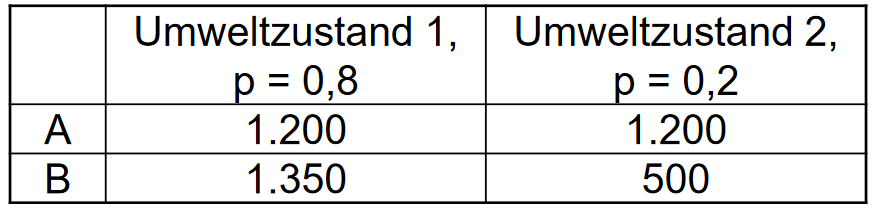
\includegraphics[width=0.4\textwidth]{images/as-1.png}
	\end{center} 
	\item Bei \underline{symmetrischer} Information: Zinssatz für A ist 10\% und für B 25\%
	\item Für Kreditnehmer wäre A bei symmetrischer Information rentabler, da
	\begin{itemize}
		\item A: $1200-1000\cdot 1,1=100$
		\item B: $0,8\cdot(1350-1000\cdot 1,25)+0,2\cdot 0=80$
	\end{itemize}
	\item \textbf{Problem}: Bank kann sich nicht sicher sein, dass A durchgeführt wird, wenn sie einen Zins von 10\% gibt. Für einen Zins $i$, den die Bank gibt, folgt für das Kalkül des Kreditnehmers:
	\begin{itemize}
		\item A: $1200-1000(1+i)=200-1000i$
		\item B: $0,8\cdot(1350-1000\cdot (1+i))+0,2\cdot 0=280-800i$
	\end{itemize}
	
	$\rightarrow$ Kreditnehmer wählt unabhängig vom Zins das Projekt B
	
	$\rightarrow$ Bank vergibt Kredite nur zu 25\% $\rightarrow$ Nur weniger effizientes Projekt B wird durchgeführt
	
	\item \textbf{Agency Kosten}: $100-80=20$ werden vom Kreditnehmer getragen 
	
	$\rightarrow$ \textbf{Lösung}: Covenants
\end{itemize}

\textbf{Moral Hazard: Verzögerte Liquidation}:
\begin{itemize}
	\item AG kann für 20 Mio. \euro\text{ }liquidiert werden, Verbindlichkeiten betragen 30 Mio. \euro
	\item Bei Fortführung wird der Wert zu 80\% auf 10 Mio. \euro\text{ } sinken und kann zu 20\% auf 40 Mio. \euro\text{ } steigen
	\item Für Eigentümer wäre Fortführung effizient, denn $0,8\cdot 0+0,2\cdot(40-30)=2\text{ Mio.}$\euro, statt 0. Für FK-Geber und Unternehmenswert aber ineffizient!
\end{itemize}
$\rightarrow$ Eigentümer haben einen Anreiz, Liquidation hinauszuzögern (\textbf{Gambling for Resurrection})\\

\textbf{Unterinvestition: Debt-Overhang Problem}:
\begin{itemize}
	\item Für Medikament werden 100 über Anleihen (Rückzahlung 105) finanziert
	\item Später eingegangene zusätzliche Verbindlichkeiten stehen im Rang hinter den Anleihegläubigern
	\item Alle Akteure risikoneutral, risikoloser Zins sei 0
	\begin{center}
		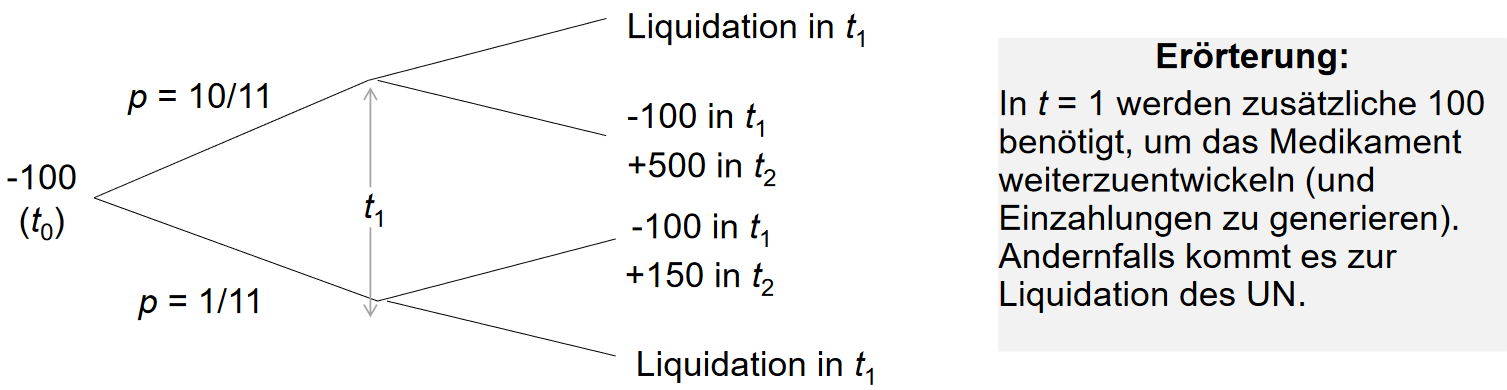
\includegraphics[width=0.7\textwidth]{images/do.png}
	\end{center} 
	\item Fall 1: Nachrangige Verbindlichkeiten können aufgenommen und zurückgezahlt werden
	\item Fall 2: Weiterentwicklung immer noch effizient, aber Finanzierung durch neue Gläubiger scheitert am Vorrang der Altverbindlichkeiten $\rightarrow$ \textbf{Debt-Overhang Problem} $\rightarrow$ Neue Kapitalgeber sind nicht bereit, ein vorteilhaftes Projekt zu finanzieren, weil Erträge den alten Gläubigern zu Gute kommen
	\item \textbf{Nachverhandlungen}: Weiterentwicklung des Produkts ist auch für Anleihegläubiger sinnvoll, da sie sonst nichts erhalten
	
	$\rightarrow$ Nachverhandlung über Senkung der Forderungshöhe von 105 auf 50 ermöglicht Projektfinanzierung durch neue Kapitalgeber
	
	\item Anleihegläubiger antizipieren \textbf{Nachverhandlungsrisiko} und fordern deshalb\\
	 $\frac{10}{11}R+\frac{1}{10}50=0\Rightarrow R=105$ als Rückzahlungsbetrag
\end{itemize}